\documentclass[final, unknownkeysallowed]{beamer}
\usetheme{RJH}
\usepackage[orientation=portrait,size=a2,scale=1.4,debug]{beamerposter}
\usepackage[absolute,overlay]{textpos}
\setlength{\TPHorizModule}{1cm}
\setlength{\TPVertModule}{1cm}

\title{Deep convolutional networks for protein structure quality assessment}
\author{Georgy Derevyanko, Guillaume Lamoureux}
\institute[CLS]{Concordia University, QC, Canada}
\footer{Footer}
\date{\today}

\begin{document}
\begin{frame}{}

\begin{textblock}{19.5}(1,5)
\begin{block}{Introduction}
Protein folding remains one of the outstanding challenges in structural biology. 
The key part of any workflow of protein structure prediction is the decoy quality assessment. 
During this step an algorithm selects the best candidate structure out of the pool of candidates. The final 
Success of the folded structure prediction largely depends on the performance of this algorithm.
\end{block}

\begin{block}{Input and model}

\begin{figure}[H]
    \centering
    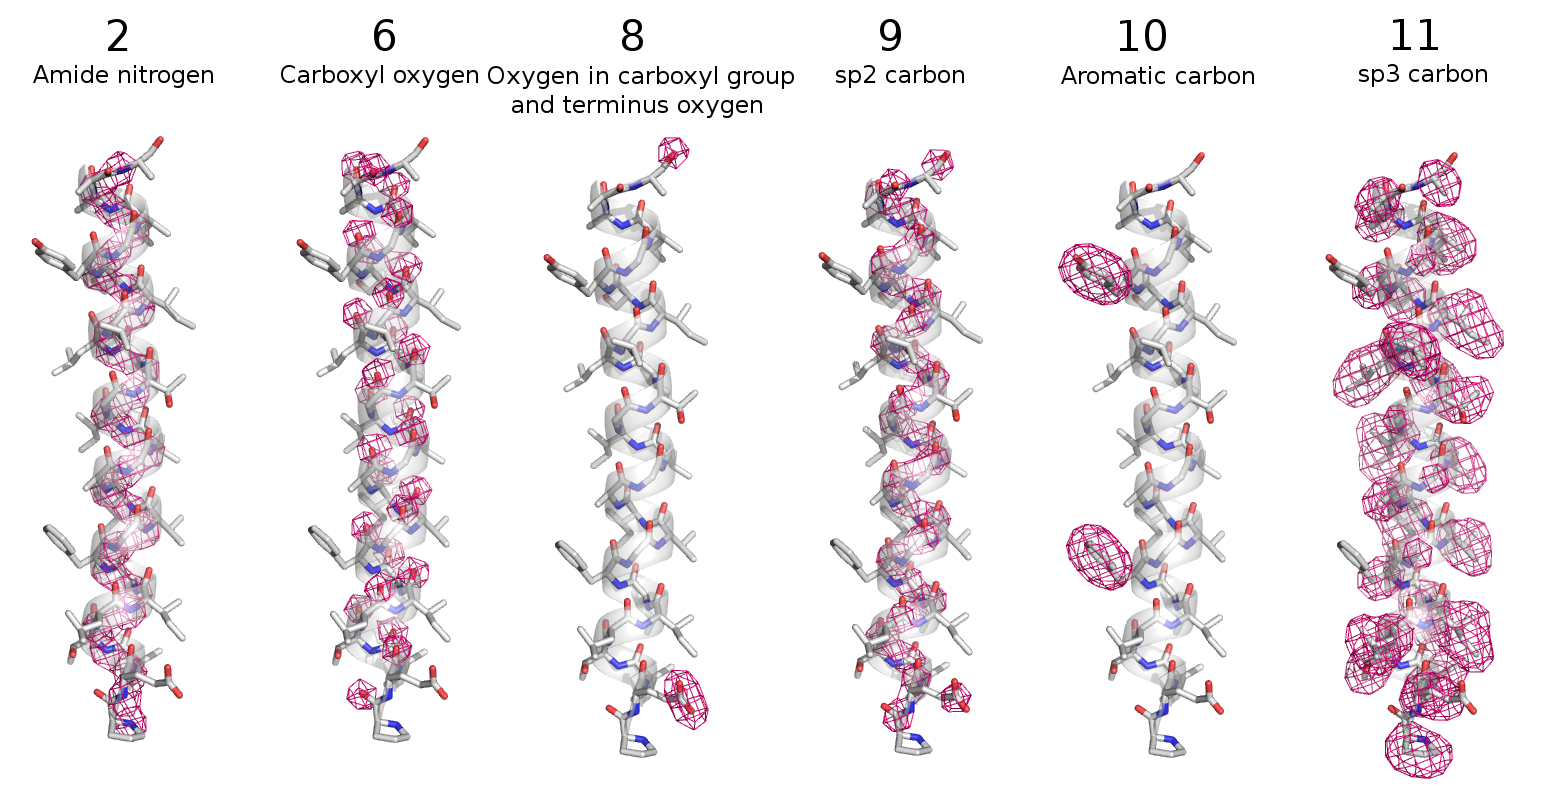
\includegraphics[width=\linewidth]{../draft/Fig/atomic_densities_V3.png}
    \caption{The example of the representation of a protein using atomic densities. The density map is 
    shown using the volumetric rendering plugin for PyMol. The pdb-code of the protein used for this visualization is 5eh6.
    The isosurface level was set to $0.5$.}
    \label{Fig:atomic_densities}
\end{figure}

\begin{figure}[H]
    \centering
    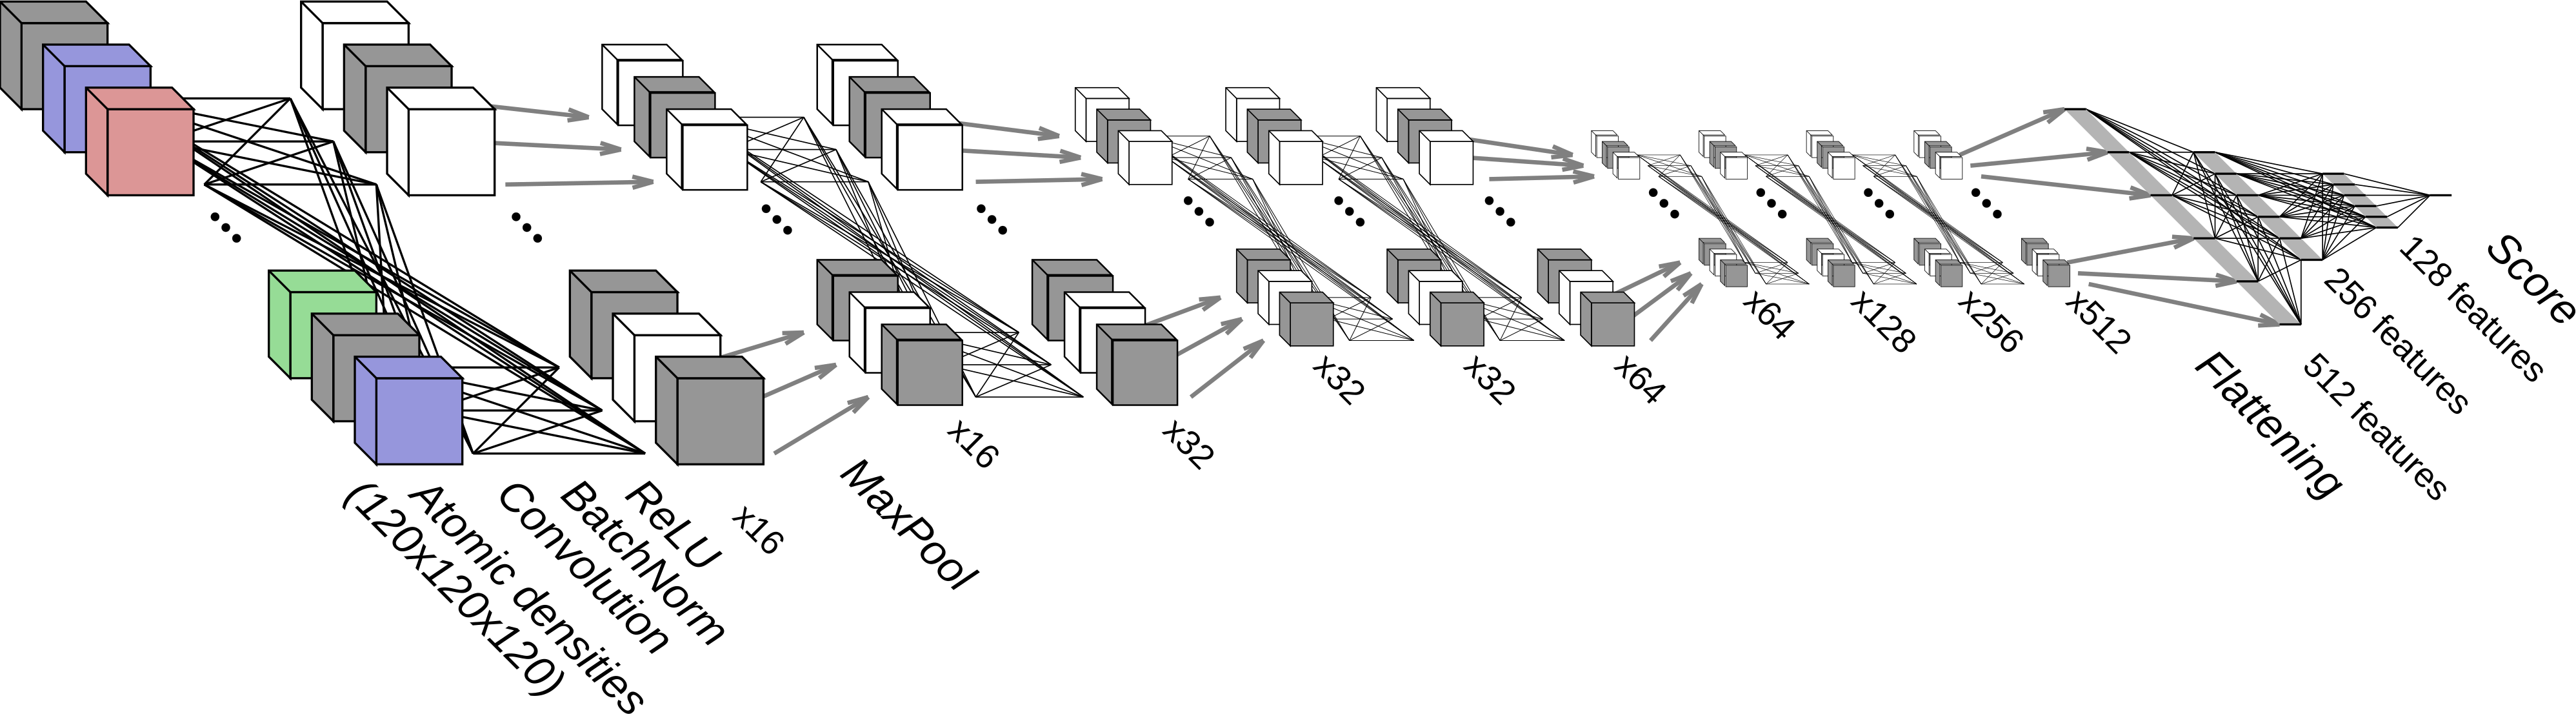
\includegraphics[width=\linewidth]{../draft/Fig/ConvnetDiagramV1.png}
    \caption{The schematic representation of the convolutional neural network architecture used in this work. 
    The arrows between the boxes denote maximum pooling layers and the connections denote 
    consequent 3d convolutional, batch normalization and ReLU layers. The numbers xM denote the number of filters 
    used in the corresponding 3d convolutional layer. The size of all filters and 
    maximum pooling domains are 3x3x3. The grey stripes denote one-dimensional vectors and crossed lines between them 
    stand for fully-connected layer with ReLU non-linearities. The details of the model parameters can be found in 
    Supplementary Information.}
    \label{Fig:CNNModel}
\end{figure}

\end{block}

\begin{block}{Datasets}
   To train and assess our method we used the datasets of protein decoys from the CASP competition \cite{moult2014critical}. 
We took the datasets CASP7 - CASP10 as the training set and the CASP11 dataset as the test set.
We optimized side chain conformation of the training and test sets using SCWRL4 program \cite{krivov2009improved}.
The training and test sets have 564 and 83 targets correspondingly. For each target the training dataset has 
on average 282 decoys. The test dataset is split into two subsets: Stage1 with 20 selected decoys for each target and Stage2 with 150 decoys
for each. The native structures were not included in the datasets nor during the training procedure
neither during the testing phase.
\begin{figure}[H]
    \makebox[\textwidth]{
    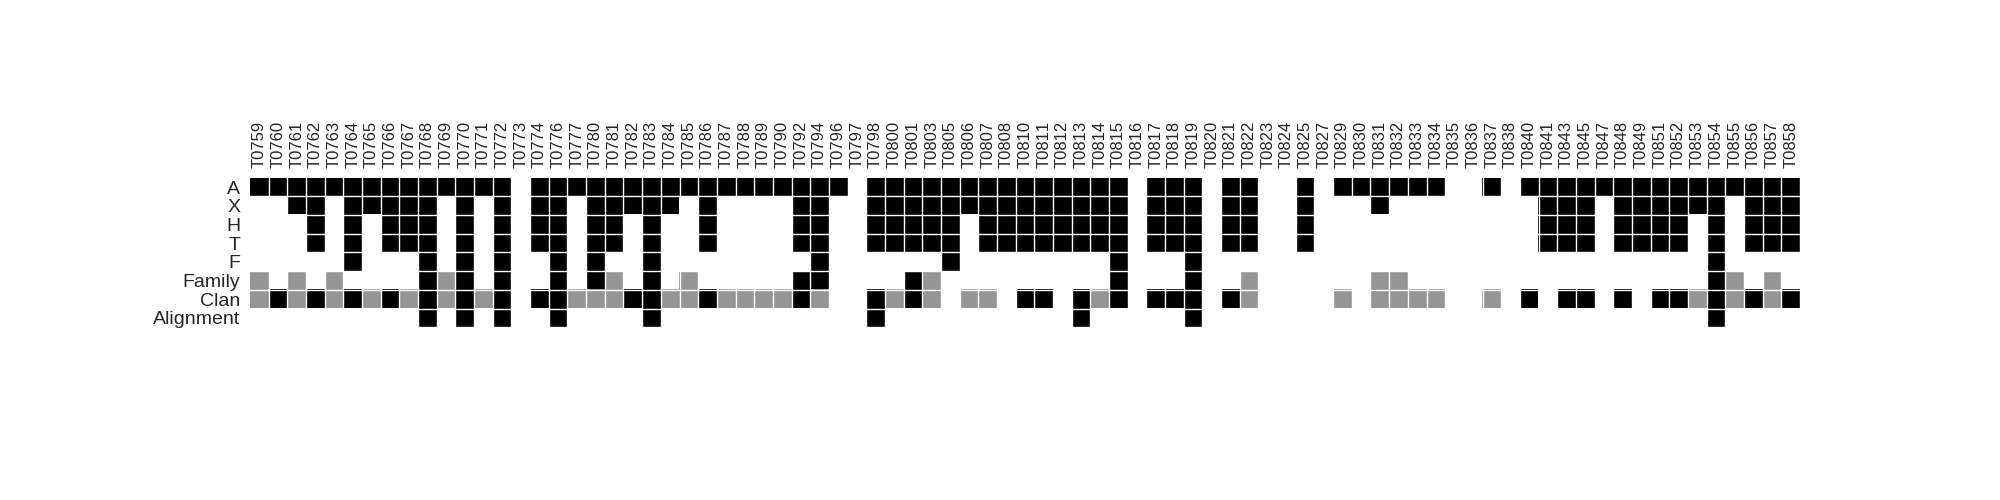
\includegraphics[width=\textwidth]{../draft/Fig/summary_table.png}
    }
%
    \caption{Overlap of the training set on each target domain of the
    test set (from T0759 to T0858). The first 5 rows of tiles
    correspond to the ECOD classification of protein domains (A-, X-,
    H-, T-, and F-groups). A black tile in any of these rows indicates
    that at least one structure from the training set belongs to the
    same ECOD group as the target. Targets for which no ECOD
    classification is available are left empty.
%%% I see that all targets excluded from the analysis have an empty
%%% row of squares. Is T0838 excluded as well? What about the targets
%%% that are not in the list? (775, 778, 779, 791, 793, 795, 799, 802,
%%% 804, 809, 826, 828, 839, 842, 844, 846, 850) Were they all
%%% excluded from the CASP competition? The CASP11 QA paper mentions
%%% that the following targets were cancelled by the organizers: 778,
%%% 779, 791, 809, 842, 844, 846, 850. What about the other ones?
    A black tile in the ``Family'' row indicates that at least one
    structure from the training set belongs to the same Pfam family as
    the target. (A grey tile indicates that no Pfam family information
    is available for the target.) The ``Clan'' row shows similar
    information for Pfam clans. A black tile in the ``Alignment'' row
    indicates that at least one sequence in the training set aligns to
    the target sequence with an E-value smaller than $10^{-4}$.}
%
    \label{Fig:summaryTable}
\end{figure}

\end{block}

\end{textblock}


\begin{textblock}{19.3}(21.8,5)

\begin{block}{Results}
The loss criterion is the deviation of the GDT-TS of the best decoys for a protein from the GDT-TS score of the decoy with the lowest score:
$$ 
Loss = | max_i( gdtts_i ) - gdtts( argmin(f(x_i) ) |
$$ 

\begin{table}[H]
\begin{center}
\begin{tabular}{ c | c | c | c | c }
    \multicolumn{5}{ c }{Stage 1} \\ \hline

    QA method & Loss & Pearson & Spearmann & Kendall \\
    \hline
    \textbf{3DCNN}   &0.071 &0.528 &0.414 &0.318 \\
    ProQ2   &0.081 &0.656 &0.534 &0.408 \\
    VoroMQA &0.095 &0.621 &0.504 &0.382 \\
    Qprob   &0.097 &0.631 &0.517 &0.389 \\
    RWplus  &0.128 &0.500 &0.387 &0.291 \\ \hline
    
    \multicolumn{5}{ c }{Stage 2} \\ \hline
    
    ProQ2   &0.058 &0.372 &0.366 &0.256 \\
    \textbf{3DCNN}   &0.067 &0.420 &0.405 &0.285 \\
    Qprob   &0.068 &0.381 &0.387 &0.272 \\
    VoroMQA &0.069 &0.444 &0.437 &0.313 \\ 
    RWplus  &0.095 &0.202 &0.246 &0.175 \\ \hline

\end{tabular}
    
    \caption {Results of our method(3DCNN) and the other state-of-art quality assessment programs on the CASP11 dataset Stage 1 and 2.
            Table shows the absolute average values of correlation coefficients. The averaging was performed for each target in the 
            dataset. Afterwards all the values were averaged over all the targets.}
    \label{Tbl:TestResults}
\end{center}
\end{table}

\end{block}

\begin{block}{Analysis}
\begin{figure}[H]
    \centering
    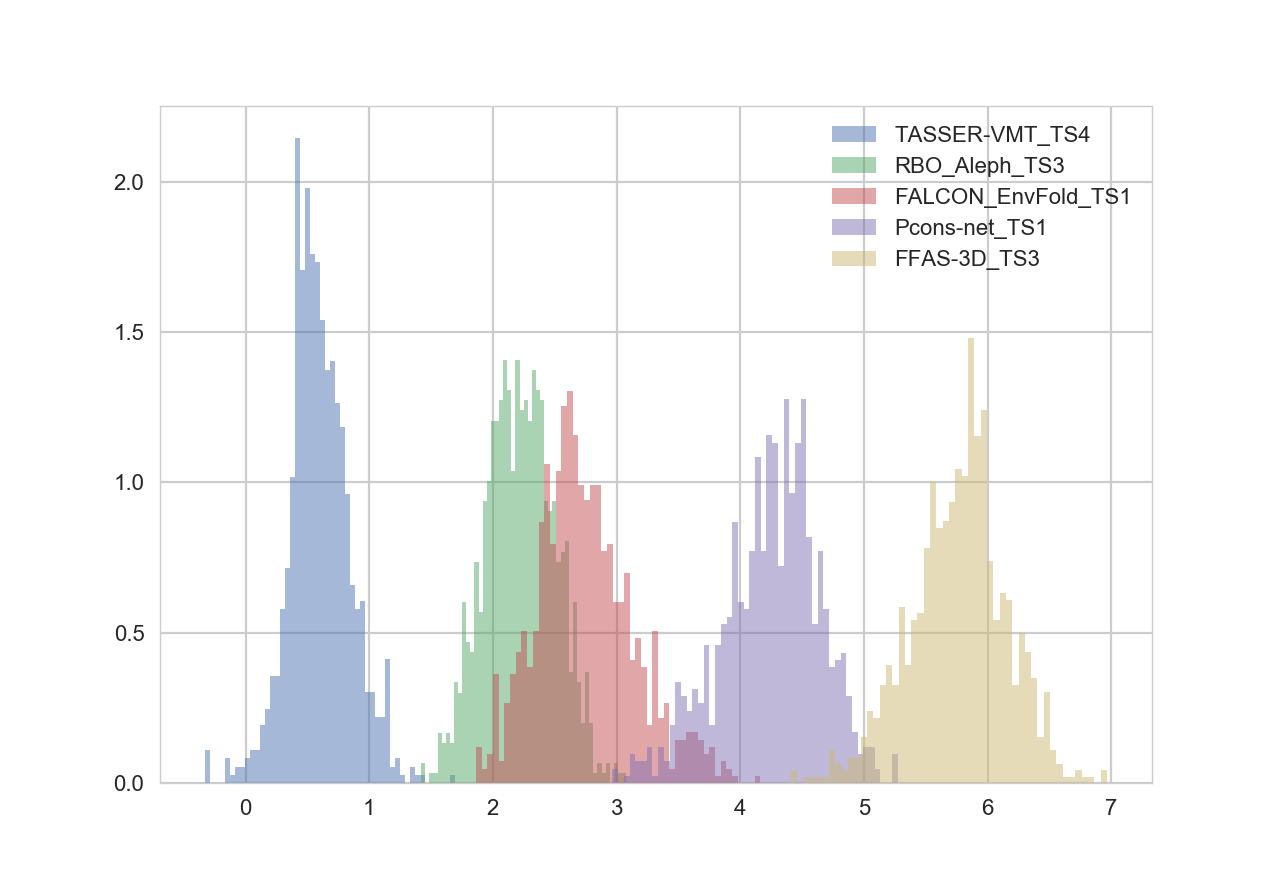
\includegraphics[width=\linewidth]{../draft/Fig/decoys_sampling_dist.png}
    \caption{The distribution of scores under random translations and rotations of several decoys for the target T0832. The 
    names arrangement from top to bottom corresponds to the increase of the score.}
    \label{Fig:DecoysScoreDistribution}
\end{figure}
\begin{figure}[H]
    \centering
    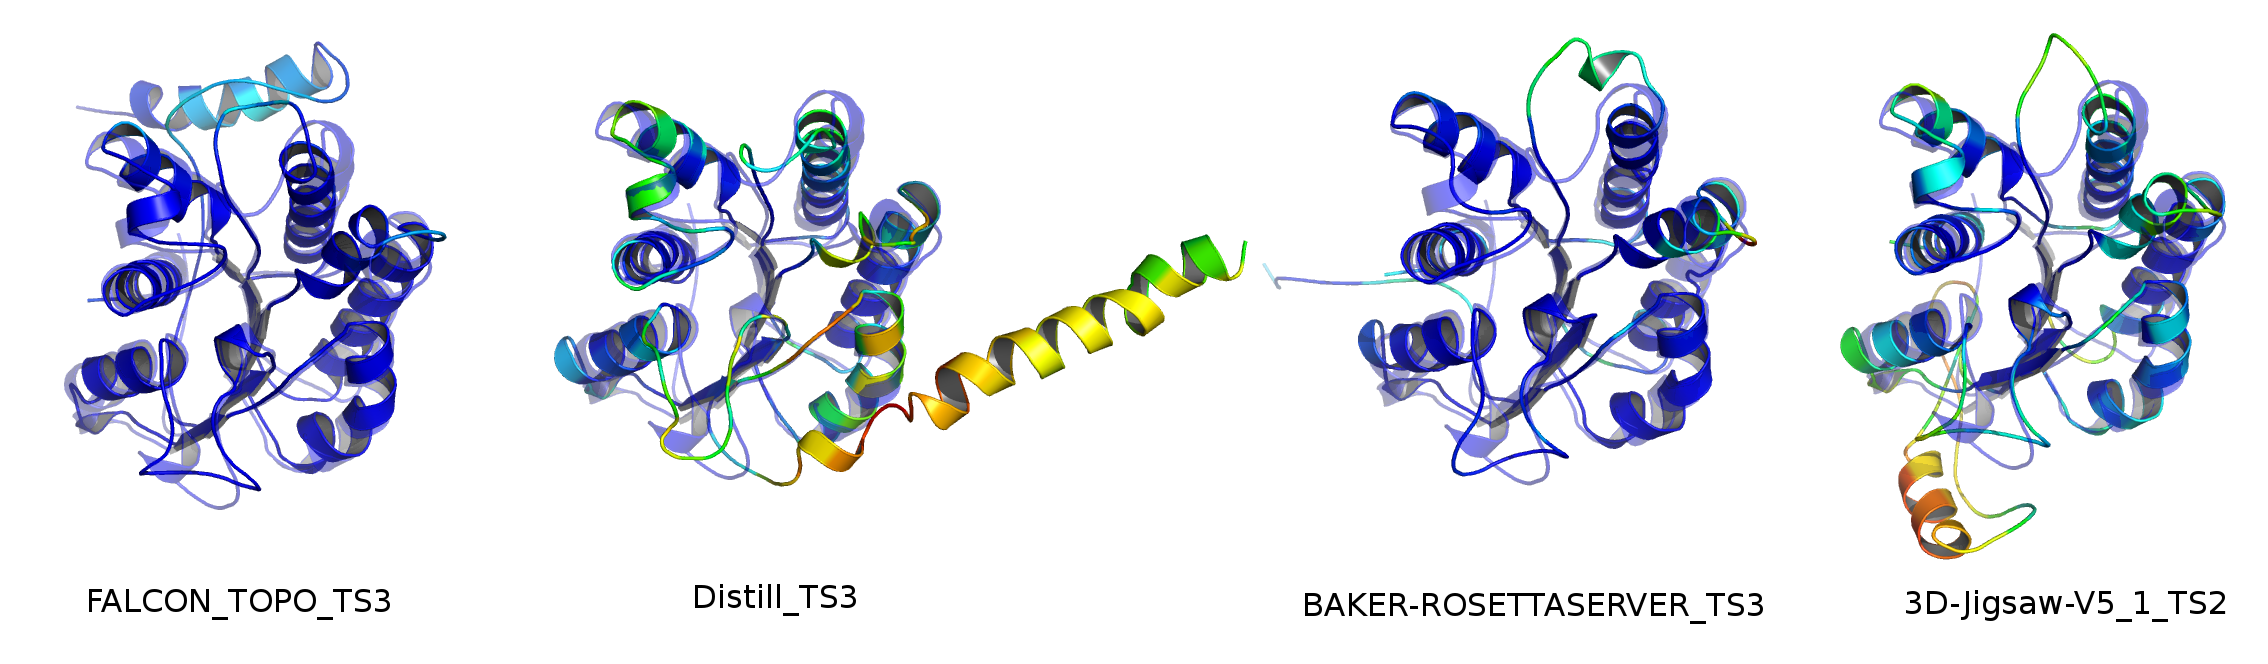
\includegraphics[width=\linewidth]{../draft/Fig/T0776.png}
    \caption{The scaled gradient weighted activation maps of the network projected onto the atoms of the decoys. 
    Each decoy is aligned to the native structure (shown with the transparent cartoon).}
    \label{Fig:GradCAMT0776_more}
\end{figure}
\end{block}


\begin{block}{Citations}
\emph{Journal of Irreproducible Results}.
\end{block}

\end{textblock}

\end{frame}
\end{document}
